% Section 3: Inner Product Spaces  (original handwritten pages 19--24)
\section{Inner Product Spaces}\label{sec:ips}
\syllabusweek{Week 4 --- inner product spaces, orthogonality, Gram--Schmidt}
\subsection{Inner Products}\label{ss:inner-products}
\begin{definition}
Let $(\V,\C)$ be a vector space. An \term{inner product} is a function from $\V\times\V$ into $\C$,
\[
\inner{\cdot}{\cdot} : \V\times\V\to\C
\]
satisfying the following properties:
\begin{enumerate}[label=\arabic*)]
\item $\inner{x}{y} = \overline{\inner{y}{x}}$ \quad $\forall x,y\in\V$ \hfill (conjugate symmetry)
\item Linearity with respect to (w.r.t.) the first argument:
  \begin{enumerate}[label=\alph*)]
  \item $\inner{x+y}{z} = \inner{x}{z} + \inner{y}{z}$ \quad $\forall x,y,z\in\V$ \hfill (additivity)
  \item $\inner{\alpha x}{y} = \alpha\inner{x}{y}$ \quad $\forall\alpha\in\C$ and $\forall x,y\in\V$ \hfill (homogeneity)
  \end{enumerate}
\item $\inner{x}{x}$ is real \& nonnegative, $\inner{x}{x}\ge 0$, and
  $\inner{x}{x} = 0 \Leftrightarrow x = 0_{\V}$ \hfill (positive definiteness)
\end{enumerate}
$\therefore$ The triplet $(\V,\C,\inner{\cdot}{\cdot})$ is called an \term{inner product space}.
\end{definition}
\begin{align*}
\inner{x}{y+z} &= \overline{\inner{y+z}{x}} = \overline{\inner{y}{x}} + \overline{\inner{z}{x}} = \inner{x}{y} + \inner{x}{z}
\end{align*}
\explain{Additivity w.r.t.\ second argument \checkmark}
\begin{align*}
\inner{x}{\alpha y} &= \overline{\inner{\alpha y}{x}} = \bar\alpha\,\overline{\inner{y}{x}} = \bar\alpha\inner{x}{y}
\end{align*}
\explain{Homogeneity w.r.t.\ second argument $\times$ ($\alpha$ should be real). We have \key{conjugate homogeneity w.r.t.\ second argument}.}
\begin{insight}
So an inner product is linear in the first argument and \emph{conjugate}-linear in the second:
$\inner{\textstyle\sum_i\alpha_i x_i}{\sum_j\beta_j y_j} = \sum_{i,j}\alpha_i\bar\beta_j\inner{x_i}{y_j}$.
Over $\F=\R$ the conjugates disappear and the inner product is bilinear and symmetric. Also $\inner{x}{0_\V} = \inner{0_\V}{x} = 0$ for all $x$ (take $\alpha = 0$ in homogeneity).
\end{insight}

% ===== Page 19 =====
\origpage{19}
\begin{example}
$\V = \C^n$, $\F = \C$, \quad
$x = [x_1\ x_2 \ldots x_n]\T$, \ $y = [y_1\ y_2 \ldots y_n]\T$, \quad $x_i, y_i\in\C$.
\[
\inner{x}{y} = \sum_{i=1}^n x_i\bar y_i = \bar y\T x = y\Hm x
\qquad \Big(\begin{bmatrix} \bar y_1 & \bar y_2 & \cdots\end{bmatrix}\bmat{x_1\\ x_2\\ \vdots}\Big)
% corrected: notes had the row vector [y_1 y_2 ...]; y^H = conj(y)^T has conjugated entries
\]
\paragraph{Check of the axioms.}
\begin{enumerate}[label=\arabic*)]
\item $\inner{x}{y} = \sum_{i=1}^n x_i\bar y_i = \bar y\T x = y\Hm x$
\[
\overline{\inner{y}{x}} = \overline{x\Hm y} = \overline{\bar x\T y} = \underbrace{x\T\bar y = \bar y\T x}_{\text{scalar} = \text{its transpose}} = y\Hm x = \inner{x}{y}
\]
\needspace{3\baselineskip}
\item \begin{enumerate}[label=\alph*)]
  \item $\inner{x+y}{z} = z\Hm(x+y) = z\Hm x + z\Hm y = \inner{x}{z} + \inner{y}{z}$
  \item $\inner{\alpha x}{y} = y\Hm(\alpha x) = \alpha y\Hm x = \alpha\inner{x}{y}$
  \end{enumerate}
\item $\inner{x}{x} = x\Hm x = \sum_{i=1}^n |x_i|^2 \ge 0 \;\Rightarrow$ real value;
  \ $\inner{x}{x} = 0 \Leftrightarrow x = 0_\V$.
\end{enumerate}
\end{example}
\begin{example}
$A, B\in\R^{m\times n}$, \ $\V=\R^{m\times n}$, \ $\F=\R$, \ $A = [a_{ij}]$, \ $B = [b_{ij}]$:
\[
\inner{A}{B} = \sum_{i,j} a_{ij}b_{ij}
\]
\[
\underbrace{\bmat{a_{11} & a_{12} & a_{13}\\ a_{21} & a_{22} & a_{23}}\cdot
\bmat{b_{11} & b_{21}\\ b_{12} & b_{22}\\ b_{13} & b_{23}}}_{A\cdot B\T}
=
\bmat{a_{11}b_{11} + a_{12}b_{12} + a_{13}b_{13} & \times\\ \times & a_{21}b_{21} + a_{22}b_{22} + a_{23}b_{23}}
\]
% corrected: notes had B^T with rows b11 b12 / b12 b22 / b13 b23 (entry (1,2) must be b21)
\begin{align*}
\inner{A}{B} &\triangleq \tr(AB\T)\\
&= \tr(A\T B) \quad \text{(in the real field)}
\end{align*}
\explain{$(AB\T)_{ii} = \sum_j a_{ij}b_{ij}$ (row $i$ of $A$ against row $i$ of $B$), so the trace adds up all $a_{ij}b_{ij}$; the off-diagonal entries ($\times$) are irrelevant. For complex matrices one uses $\inner{A}{B} = \tr(AB\Hm) = \tr(B\Hm A)$, whose induced norm is the Frobenius norm.}
\end{example}
\begin{example}
$\V = \left\{ f(\cdot) \;\middle|\; f:[0,1]\to\C \text{ s.t. } \int_0^1 |f(t)|^2\,dt < \infty\right\}$
\[
\inner{f_1}{f_2} \triangleq \int_0^1 f_1(t)\overline{f_2(t)}\,dt \qquad (\mathcal{L}_2 \text{ inner product})
\]
\end{example}
\subsection{The Cauchy--Schwarz Inequality and the Induced Norm}\label{ss:cauchy-schwarz}
\begin{theorem}[Cauchy--Schwarz Inequality]
Let $\V$ be an inner product space. Let $x,y\in\V$.
\[
|\inner{x}{y}|^2 \le \inner{x}{x}\inner{y}{y}
\]
Equality holds iff $x = cy$ for some $c\in\C$ or $y = 0_\V$, i.e.\ \key{equality iff $x$ and $y$ are linearly dependent}.
\end{theorem}
% corrected: notes stated equality iff x = cy; the case y = 0_V (x arbitrary) also gives equality 0 = 0, so the condition is linear dependence
\paragraph{Equality check for $x = cy$.}
\begin{align*}
\inner{x}{y} &= \inner{cy}{y} = c\inner{y}{y} \;\Rightarrow\; |\inner{x}{y}|^2 = |c|^2\inner{y}{y}^2\\
\inner{x}{x} &= \inner{cy}{cy} = c\bar c\inner{y}{y} = |c|^2\inner{y}{y} \qquad (c\bar c = |c|^2 \text{ is real})
\end{align*}
\explain{Using the first- and second-argument axioms.}
\[
\underbrace{|c|^2\inner{y}{y}^2}_{|\inner{x}{y}|^2} = \underbrace{|c|^2\inner{y}{y}}_{\inner{x}{x}}\underbrace{\inner{y}{y}}_{\inner{y}{y}}
\]

% ===== Page 20 =====
\origpage{20}
\needspace{6\baselineskip}
\begin{proof}[Proof of theorem]
We distinguish two cases.
\paragraph{Case 1: $y = 0_{\V}$.}
\begin{align*}
\inner{x}{y} &= \inner{x}{0_{\V}} = \inner{x}{0\cdot 0_{\V}} = 0\cdot\inner{x}{0_{\V}} = 0\\
\inner{y}{y} &= 0 \quad \text{(by axioms)}\\
\underbrace{|\inner{x}{y}|^2}_{0} &\le \underbrace{\inner{x}{x}}_{\ge 0}\underbrace{\inner{y}{y}}_{0} \;\Rightarrow\; 0\le 0 \ \checkmark
\end{align*}
\paragraph{Case 2: $y\neq 0_{\V}$.} Then $\inner{y}{y}\neq 0$ (in fact $\inner{y}{y}>0$ by axiom 3, so we may divide by it and multiply inequalities by it).
For $\alpha\in\C$ (in field):
\begin{align*}
0 &\le \inner{x-\alpha y}{x-\alpha y}\\
&= \inner{x}{x} - \inner{x}{\alpha y} - \inner{\alpha y}{x} + \inner{\alpha y}{\alpha y}\\
&= \inner{x}{x} - \bar\alpha\inner{x}{y} - \alpha{\underbrace{\inner{y}{x}}_{\overline{\inner{x}{y}}}} + |\alpha|^2\inner{y}{y}
\end{align*}
Choose $\displaystyle \alpha = \frac{\inner{x}{y}}{\inner{y}{y}}$:
\begin{align*}
0 &\le \inner{x}{x} - \frac{\overline{\inner{x}{y}}}{\inner{y}{y}}\cdot\inner{x}{y} - \cancel{\frac{\inner{x}{y}}{\inner{y}{y}}\cdot\overline{\inner{x}{y}}} + \cancel{\frac{|\inner{x}{y}|^2}{\inner{y}{y}^2}\cdot\inner{y}{y}}\\
0 &\le \inner{x}{x} - \frac{|\inner{x}{y}|^2}{\inner{y}{y}}\\
\frac{|\inner{x}{y}|^2}{\inner{y}{y}} &\le \inner{x}{x} \;\Rightarrow\; \therefore\ |\inner{x}{y}|^2 \le \inner{x}{x}\inner{y}{y}
\qedhere
\end{align*}
\end{proof}
\begin{insight}[Choice of $\alpha$ and the equality case]
$\alpha y$ with $\alpha = \inner{x}{y}/\inner{y}{y}$ is the projection of $x$ onto $y$ (see Gram--Schmidt below), so $x-\alpha y\perp y$ and the first line says $\norm{x-\alpha y}^2\ge 0$: the error of the best approximation of $x$ along $y$ has nonnegative length.
Equality in the theorem (with $y\neq 0_\V$) holds iff $\inner{x-\alpha y}{x-\alpha y} = 0$, i.e.\ iff $x = \alpha y$ by axiom 3. This proves the ``only if'' part of the equality statement; the ``if'' part is the check for $x = cy$ above.
\end{insight}

\begin{remark}
An inner product \key{induces a norm} (the \term{induced norm}) defined as
\[
\norm{x}^2 \triangleq \inner{x}{x}, \qquad \norm{x} \triangleq \sqrt{\inner{x}{x}}
\]
\end{remark}
\paragraph{Show that this is a norm.}
\begin{enumerate}[label=\arabic*)]
\item $\norm{x}\ge 0$, \ $\norm{x} = 0 \Leftrightarrow x = 0_{\V}$ \checkmark \ (by axiom 3 of the inner product) \hfill (positive definiteness)
\item $\displaystyle \norm{\alpha x} \triangleq \sqrt{\inner{\alpha x}{\alpha x}} = \sqrt{\alpha\cdot\bar\alpha\inner{x}{x}}
= |\alpha|\underbrace{\sqrt{\inner{x}{x}}}_{\norm{x}} = |\alpha|\norm{x}$ \checkmark \hfill (absolute homogeneity)
\item $\norm{x+y} = \sqrt{\inner{x+y}{x+y}}$ \hfill (triangle inequality)
\begin{align*}
\norm{x+y}^2 &= \inner{x+y}{x+y} = \inner{x}{x} + \inner{x}{y} + {\underbrace{\inner{y}{x}}_{\overline{\inner{x}{y}}}} + \inner{y}{y}\\
&= \inner{x}{x} + 2\cdot\operatorname{Re}\inner{x}{y} + \inner{y}{y}\\
&\le \inner{x}{x} + 2|\operatorname{Re}\inner{x}{y}| + \inner{y}{y}\\
&\le \inner{x}{x} + 2|\inner{x}{y}| + \inner{y}{y}
\intertext{\origpage{21}By Cauchy--Schwarz, $|\inner{x}{y}| \le \sqrt{\inner{x}{x}\inner{y}{y}}$:}
% ===== Page 21 =====
&\le \inner{x}{x} + 2\sqrt{\inner{x}{x}}\sqrt{\inner{y}{y}} + \inner{y}{y}\\*
&= \left(\sqrt{\inner{x}{x}} + \sqrt{\inner{y}{y}}\right)^2\\*
&= (\norm{x} + \norm{y})^2\\*
\norm{x+y}^2 &\le (\norm{x} + \norm{y})^2 \;\Rightarrow\; \norm{x+y}\le\norm{x}+\norm{y} \ \checkmark
\end{align*}
\explain{Both sides are nonnegative, so taking square roots preserves the inequality: the triangle inequality holds.}
\end{enumerate}

\sep
\paragraph{Angle between vectors.} By Cauchy--Schwarz, $|\inner{x}{y}| \le \norm{x}\norm{y}$; \ suppose $x\neq 0_{\V}$, $y\neq 0_{\V}$:
\[
0 \le \frac{|\inner{x}{y}|}{\norm{x}\norm{y}} \le 1
\]
\[
\cos\theta \triangleq \frac{|\inner{x}{y}|}{\norm{x}\norm{y}} \;\Rightarrow\; \theta = \arccos\left(\frac{|\inner{x}{y}|}{\norm{x}\norm{y}}\right)
\]
\explain{Cauchy--Schwarz is exactly what makes this angle well defined. With the absolute value $\theta\in[0,\frac\pi2]$; in a real space one often drops it, $\cos\theta = \frac{\inner{x}{y}}{\norm{x}\norm{y}}\in[-1,1]$, which for $\R^2,\R^3$ is the usual geometric angle. $\theta = \frac\pi2$ $\Leftrightarrow$ $\inner{x}{y}=0$ (orthogonal), $\theta = 0$ $\Leftrightarrow$ $x = cy$.}
\begin{remark}
\key{Every inner product space is also a normed space.} The converse/reverse is not correct in general.
\end{remark}
\begin{insight}
A norm comes from an inner product \key{iff it satisfies the parallelogram law}
$\norm{x+y}^2 + \norm{x-y}^2 = 2\norm{x}^2 + 2\norm{y}^2$.
For example $\norm{\cdot}_1$ on $\R^2$ fails it: $x = e_1$, $y = e_2$ give $4+4 = 8 \neq 4 = 2+2$. So $\ell_1$ and $\ell_\infty$ are norms without an inner product behind them; only $\ell_2$ is induced by $\inner{x}{y} = y\T x$.
\end{insight}
\begin{definition}
An inner product space that is complete w.r.t.\ the induced norm is called a \term{complete inner product space} / \term{Hilbert space}.
\end{definition}
\subsection{Orthogonality and Orthogonal Expansions}\label{ss:orthogonality}
\begin{definition}
Two vectors $x,y\in\V$ are said to be \term{orthogonal} iff $\inner{x}{y} = 0$.
Similarly subsets $S_1, S_2\subset\V$ are orthogonal iff $\inner{x}{y} = 0$ $\forall x\in S_1$, $\forall y\in S_2$.
\end{definition}
\needspace{9\baselineskip}
\paragraph{Examples.}
\begin{enumerate}[label=\arabic*)]
\item $\V=\R^n$, $\F=\R$, \quad $\inner{x}{y} = \sum_{i=1}^n x_iy_i = y\T x = x\T y$
\[
\underbrace{B = \{e_1, e_2, \ldots, e_n\}}_{\text{canonical basis set}} \qquad
e_1 = \bmat{1\\ 0\\ \vdots\\ 0} \quad e_2 = \bmat{0\\ 1\\ 0\\ \vdots\\ 0} \quad \cdots
\]
\[
\inner{e_i}{e_j} = \begin{cases} 0, & i\neq j\\ 1, & i = j\end{cases} = \delta_{ij}
\]
\item $\V = \left\{ f(\cdot) \;\middle|\; f:[-\pi,\pi]\to\C \text{ s.t. } \int_{-\pi}^{\pi}|f(t)|^2\,dt < \infty\right\}$

Consider $\{e^{jnt}\}_{n=-\infty}^{\infty}$, \quad $e^{jnt}\in\V$ for all $n$.
\[
\inner{f_1(t)}{f_2(t)} = \int_{-\pi}^{\pi} f_1(t)\,\overline{f_2(t)}\,dt
\]
\begin{align*}
\inner{e^{jnt}}{e^{jmt}} &= \int_{-\pi}^{\pi} e^{jnt}\,e^{-jmt}\,dt = \int_{-\pi}^{\pi} e^{j(n-m)t}\,dt\\
&= \int_{-\pi}^{\pi}\big[\cos((n-m)t) + j\sin((n-m)t)\big]\,dt\\
% ===== Page 22 =====
&= \int_{-\pi}^{\pi}\cos((n-m)t)\,dt + j\underbrace{\cancel{\int_{-\pi}^{\pi}\sin((n-m)t)\,dt}}_{0}
\end{align*}
\origpage{22}
\begin{center}
\begin{minipage}{0.5\textwidth}
\small $\left.\begin{array}{l}\sin t\\ \sin 2t\\ \sin 3t\\ \ \vdots\end{array}\right\}$ all zero due to integral over a period
\end{minipage}%
\begin{minipage}{0.35\textwidth}
\centering
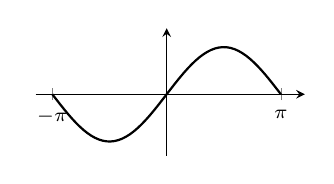
\begin{tikzpicture}
\begin{axis}[width=5cm,height=3.2cm,axis lines=middle,
  xmin=-3.6,xmax=3.8,ymin=-1.3,ymax=1.4,xtick={-3.1416,3.1416},xticklabels={$-\pi$,$\pi$},
  ytick=\empty,tick label style={font=\scriptsize}]
  \addplot[thick,domain=-pi:pi,samples=60] {sin(deg(x))};
\end{axis}
\end{tikzpicture}
\end{minipage}
\end{center}
\begin{align*}
\inner{e^{jnt}}{e^{jmt}} &= \begin{cases} 2\pi, & n = m\\ 0, & n\neq m\end{cases}\\
&= 2\pi\,\delta_{nm}
\end{align*}
\explain{For $n=m$: $\int_{-\pi}^{\pi}\cos 0\,dt = 2\pi$. For $k = n-m\neq0$: $\int_{-\pi}^{\pi}\cos kt\,dt = \frac{2\sin k\pi}{k} = 0$, and $\int_{-\pi}^{\pi}\sin kt\,dt = 0$ since $\sin kt$ is odd.}
\item $S_1 = \{\sin nt\}_{n=1}^\infty$, \ $S_2 = \{\cos mt\}_{m=1}^\infty$:
\begin{align*}
\inner{\sin nt}{\cos mt} &= \int_{-\pi}^{\pi}\sin nt\cdot\cos mt\,dt\\
&= \int_{-\pi}^{\pi}\frac12\Big(\underbrace{\cancel{\sin((n+m)t)}}_{0} + \underbrace{\cancel{\sin((n-m)t)}}_{0}\Big)\,dt = 0
\end{align*}
\explain{Product-to-sum: $\sin a\cos b = \frac12[\sin(a+b)+\sin(a-b)]$; both terms are odd functions (or zero when $n=m$), so they integrate to $0$ over the symmetric interval $[-\pi,\pi]$.}
\[
\therefore\ \key{$S_1\perp S_2$}
\]
\end{enumerate}

\sep
\paragraph{Expansion in an orthogonal set.}
\begin{itemize}
\item $z = \alpha_1 z_1 + \alpha_2 z_2$ \quad if $z_1\perp z_2$:
\begin{align*}
\inner{z}{z_1} &= \inner{\alpha_1 z_1 + \alpha_2 z_2}{z_1}\\
&= \alpha_1\inner{z_1}{z_1} + \alpha_2\underbrace{\cancel{\inner{z_2}{z_1}}}_{0} \;\Rightarrow\; \alpha_1 = \frac{\inner{z}{z_1}}{\inner{z_1}{z_1}}
\end{align*}
In general,
\[
z = \sum_{i=1}^n \alpha_i z_i, \qquad \alpha_i = \frac{\inner{z}{z_i}}{\inner{z_i}{z_i}} \quad \forall i
\]
\explain{Valid when $z\in\Span\{z_1,\ldots,z_n\}$ and the $z_i\neq 0_\V$ are mutually orthogonal: take $\inner{\cdot}{z_k}$ of both sides and all terms with $i\neq k$ vanish. \key{No linear system has to be solved; each coefficient is computed independently.}}
\paragraph{Example (as $z_1\perp z_2$).}
\[
{\underbrace{\bmat{2\\ 3}}_{z}} = \beta_1{\underbrace{\bmat{1\\ 1}}_{z_1}} + \beta_2{\underbrace{\bmat{1\\ -1}}_{z_2}},
\qquad
\beta_1 = \frac{\inner{z}{z_1}}{\inner{z_1}{z_1}} = \frac{5}{2},
\qquad
\beta_2 = \frac{\inner{z}{z_2}}{\inner{z_2}{z_2}} = \frac{2-3}{2} = -\frac12
\]
\explain{Check: $\frac52\bmat{1\\1} - \frac12\bmat{1\\-1} = \bmat{2\\3}$ \checkmark}
\item $f(t) = \sum_{n=-\infty}^{\infty}\alpha_n e^{jnt}$:
\[
\alpha_n = \frac{\inner{f(t)}{e^{jnt}}}{\inner{e^{jnt}}{e^{jnt}}} = \frac{1}{2\pi}\int_{-\pi}^{\pi} f(t)e^{-jnt}\,dt \qquad \text{(Fourier series coefficients)}
\]
\explain{With $\inner{f_1}{f_2} = \int_{-\pi}^{\pi} f_1(t)\,\overline{f_2(t)}\,dt$.}
\end{itemize}

% ===== Page 23 =====
\subsection{Gram--Schmidt Orthogonalization}\label{ss:gram-schmidt}
\origpage{23}%
\paragraph{Question.} Let $\V$ be an inner product space. Let $S_1 = \{v_1, v_2, \ldots, v_n\}$ be a linearly independent set. Can we obtain another set $S_2 = \{w_1, w_2, \ldots, w_n\}$ such that
\begin{enumerate}[label=\arabic*)]
\item $w_i\perp w_j$ when $i\neq j$
\item $\Span\{S_1\} = \Span\{S_2\}$?
\end{enumerate}
\key{Yes!} (constructively, by the following algorithm)

\needspace{9\baselineskip}
\paragraph{Gram--Schmidt orthogonalization algorithm.} The $w_k$ are constructed one at a time.
\paragraph{Step 1.} $w_1 = v_1$

\paragraph{Step 2.} $\displaystyle w_2 = v_2 - \frac{\inner{v_2}{w_1}}{\inner{w_1}{w_1}}\cdot w_1$
\begin{align*}
\inner{w_2}{w_1} &= \inner{v_2 - \frac{\inner{v_2}{w_1}}{\inner{w_1}{w_1}}\cdot w_1}{w_1}\\
&= \cancel{\inner{v_2}{w_1}} - \underbrace{\frac{\cancel{\inner{v_2}{w_1}}}{\cancel{\inner{w_1}{w_1}}}}_{\text{scalar}}\cancel{\inner{w_1}{w_1}} = 0
\end{align*}
\begin{center}
\begin{minipage}{0.55\textwidth}
\centering
\begin{tikzpicture}[scale=1.5]
  \coordinate (O) at (0,0);
  \coordinate (V1) at (1,2.4);
  \coordinate (V2) at (2.6,0.7);
  % projection of v2 onto v1: k = <v2,v1>/<v1,v1>
  \pgfmathsetmacro{\k}{(1*2.6+2.4*0.7)/(1*1+2.4*2.4)}
  \coordinate (P) at ({\k*1},{\k*2.4});
  \draw[->,thick,blue!60!black] (O) -- (V1) node[above] {$v_1 = w_1$};
  \draw[->,thick] (O) -- (V2) node[right] {$v_2$};
  \draw[->,very thick,red!60!black] (O) -- (P);
  \draw[->,very thick,red!80!black] (O) -- ($(O)!0.42!(P)$);
  \node[red!60!black,left,font=\small] at ($(O)!0.25!(P)+(-0.05,0)$) {$\frac{w_1}{\norm{w_1}}$};
  \draw[->,thick] (P) -- (V2) node[midway,above right] {$w_2$};
  \draw[dashed,red!60!black] (P) -- (V2);
  % right-angle mark at P
  \draw ($(P)!0.12cm!(V2)$) -- ($(P)!0.12cm!(V2)+(P)!0.12cm!(V1)-(P)$) -- ($(P)!0.12cm!(V1)$);
  \node[red!60!black,left,font=\small] at ($(P)+(-0.45,0.25)$) {$\frac{\inner{v_2}{w_1}}{\inner{w_1}{w_1}}\cdot w_1$};
  \draw[->,red!60!black] ($(P)+(-0.5,0.2)$) -- ($(P)+(-0.05,0.02)$);
  \pic[draw,"$\theta$",angle radius=0.45cm,angle eccentricity=1.45] {angle = V2--O--V1};
\end{tikzpicture}
\end{minipage}%
\begin{minipage}{0.4\textwidth}
\[
\inner{x}{y} = \norm{x}\norm{y}\cos\theta
\]
\end{minipage}
\end{center}
\[
\frac{\inner{v_2}{w_1}}{\underbrace{\inner{w_1}{w_1}}_{\norm{w_1}^2}}\cdot w_1
= \frac{\inner{v_2}{w_1}}{\norm{w_1}}\cdot\frac{w_1}{\norm{w_1}}
= \underbrace{\inner{v_2}{\frac{w_1}{\norm{w_1}}}}_{\norm{v_2}\cos\theta}\frac{w_1}{\norm{w_1}}
\]

\paragraph{Step 3.} $\displaystyle w_3 = v_3 - \frac{\inner{v_3}{w_1}}{\inner{w_1}{w_1}}\cdot w_1 - \frac{\inner{v_3}{w_2}}{\inner{w_2}{w_2}}\cdot w_2$
\[
\frac{\inner{v_i}{w_j}}{\inner{w_j}{w_j}}\cdot w_j \;:\; \text{\term{projection} of } v_i \text{ onto } w_j
\]

\paragraph{Step $n$.} $\displaystyle w_n = v_n - \sum_{i=1}^{n-1}\frac{\inner{v_n}{w_i}}{\inner{w_i}{w_i}}\cdot w_i$
\begin{insight}[Why Gram--Schmidt works]
\emph{Orthogonality} (by induction): if $w_1,\ldots,w_{k-1}$ are mutually orthogonal, then for $j<k$
$\inner{w_k}{w_j} = \inner{v_k}{w_j} - \sum_{i<k}\frac{\inner{v_k}{w_i}}{\inner{w_i}{w_i}}\inner{w_i}{w_j} = \inner{v_k}{w_j} - \inner{v_k}{w_j} = 0$,
since only the $i=j$ term survives.
\emph{Same span}: each $w_k$ is $v_k$ minus a combination of $w_1,\ldots,w_{k-1}\in\Span\{v_1,\ldots,v_{k-1}\}$, so $\Span\{w_1,\ldots,w_k\} = \Span\{v_1,\ldots,v_k\}$ for every $k$.
\emph{No division by zero}: $w_k = 0_\V$ would make $v_k\in\Span\{v_1,\ldots,v_{k-1}\}$, impossible for a linearly independent $S_1$; so $\inner{w_k}{w_k}>0$.
In words: \key{$w_k$ is the component of $v_k$ orthogonal to the span of the previous vectors.}
\end{insight}

\begin{example}
$\V = \left\{ f \;\middle|\; f:[-1,1]\to\R,\ \int_{-1}^{1}(f(t))^2\,dt < \infty\right\}$, \quad $\F = \R$,
\[
\inner{f}{g} = \int_{-1}^{1} f(t)g(t)\,dt
\]
\[
S_1 = \{v_1, v_2, v_3\}, \qquad v_1(t) = 1, \quad v_2(t) = t, \quad v_3(t) = t^2,
\qquad\text{i.e.}\quad S_1 = \{1, t, t^2\}
\]

% ===== Page 24 =====
\origpage{24}
\begin{align*}
w_1 &= v_1 = 1\\
w_2 &= t - \frac{\overset{0}{\cancel{\inner{t}{1}}}}{\inner{1}{1}}\cdot 1 = t, \qquad \inner{t}{1} = \int_{-1}^{1} t\,dt = 0\\
w_3 &= t^2 - \frac{\inner{t^2}{1}}{\inner{1}{1}}\cdot 1 - \frac{\overset{0}{\cancel{\inner{t^2}{t}}}}{\inner{t}{t}}\cdot t = t^2 - \frac{2/3}{2} = t^2 - \frac13
\end{align*}
using
\begin{align*}
\inner{t^2}{1} &= \int_{-1}^{1} t^2\,dt = 2\int_0^1 t^2\,dt = \frac23\\
\inner{1}{1} &= \int_{-1}^{1} 1\,dt = 2\\
\inner{t^2}{t} &= \int_{-1}^{1} t^3\,dt = 0\\
\inner{t}{t} &= \int_{-1}^{1} t^2\,dt = \frac23
\end{align*}
\begin{center}
\begin{minipage}{0.45\textwidth}
\[
S_2 = \left\{1,\ t,\ t^2 - \tfrac13\right\}
\]
\centering \term{Legendre polynomials}
\end{minipage}%
\begin{minipage}{0.5\textwidth}
\centering
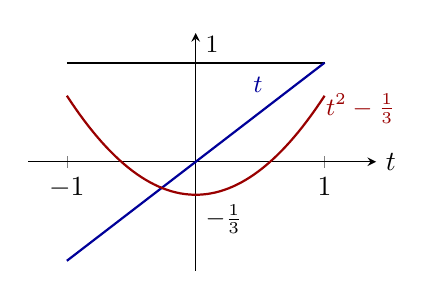
\begin{tikzpicture}
\begin{axis}[width=6cm,height=4.6cm,axis lines=middle,
  xmin=-1.3,xmax=1.4,ymin=-1.1,ymax=1.3,xtick={-1,1},ytick=\empty,xlabel={$t$},
  every axis x label/.style={at={(current axis.right of origin)},anchor=west},clip=false]
  \addplot[thick,domain=-1:1] {1};
  \node[above right,font=\small] at (axis cs:0,1) {$1$};
  \node[below right,font=\small] at (axis cs:0,-0.3333) {$-\frac13$};
  \addplot[thick,domain=-1:1,blue!60!black] {x} node[pos=0.8,above left,font=\small] {$t$};
  \addplot[thick,domain=-1:1,samples=60,red!60!black] {x^2-1/3} node[pos=0.95,right,font=\small] {$t^2-\frac13$};
\end{axis}
\end{tikzpicture}
\end{minipage}
\end{center}
\explain{Check: $\inner{t^2-\frac13}{1} = \frac23 - \frac13\cdot 2 = 0$ and $\inner{t^2-\frac13}{t} = \int_{-1}^1 (t^3 - \frac t3)\,dt = 0$ (odd integrand) \checkmark. These are the Legendre polynomials up to scaling: the standard ones are $P_0 = 1$, $P_1 = t$, $P_2 = \frac12(3t^2-1) = \frac32\big(t^2-\frac13\big)$, normalised so that $P_k(1) = 1$.}
\end{example}

\needspace{9\baselineskip}
\sep
\paragraph{Linearly dependent vectors.} If the vectors are linearly dependent, e.g.\ $S_1 = \{v_1, v_1\}$:
\begin{align*}
w_1 &= v_1\\
w_2 &= v_1 - \frac{\overset{1}{\cancel{\inner{v_1}{v_1}}}}{\cancel{\inner{v_1}{v_1}}}\cdot v_1 = 0
\end{align*}
\explain{When this is the case, \key{remove the redundant vector and resume the process}. In general $w_k = 0_\V$ exactly when $v_k$ depends linearly on $v_1,\ldots,v_{k-1}$; discarding such vectors, Gram--Schmidt returns an orthogonal basis of $\Span\{S_1\}$ (and its size is $\dim\Span\{S_1\}$).}

\needspace{12\baselineskip}
\paragraph{Gram--Schmidt orthonormalization.}
Require $\norm{w_i} = 1$, i.e.\ $\inner{w_i}{w_i} = 1$:
\begin{alignat*}{2}
\bar w_1 &= v_1, &\qquad w_1 &= \frac{\bar w_1}{\norm{\bar w_1}}\\*
\bar w_2 &= v_2 - \inner{v_2}{w_1}w_1, &\qquad w_2 &= \frac{\bar w_2}{\norm{\bar w_2}}\\*
&\ \,\vdots\\*
\bar w_n &= v_n - \sum_{i=1}^{n-1}\inner{v_n}{w_i}w_i, &\qquad w_n &= \frac{\bar w_n}{\norm{\bar w_n}}
\end{alignat*}
% corrected: notes had w_2 = \bar w_2 / ||w_2||; the normalisation divides by ||\bar w_2||. The last normalisation w_n = \bar w_n/||\bar w_n|| is implied by the pattern and added.
\explain{Since $\inner{w_i}{w_i} = 1$, the projection coefficients $\frac{\inner{v_k}{w_i}}{\inner{w_i}{w_i}}$ simplify to $\inner{v_k}{w_i}$. The resulting set is \term{orthonormal}: $\inner{w_i}{w_j} = \delta_{ij}$.}
